\section{INTRODUÇÃO}

Em decorrência da popularização dos veículos de carroceria fechada, constatou-se a necessidade do desenvolvimento de sistemas voltados à garantia do conforto térmico de seus ocupantes. 
Assim, na década de 1930, iniciou-se nos Estados Unidos o desenvolvimento do sistema de condicionamento de ar em veículos, com o primeiro registro de comercialização do primeiro veículo com sistema de condicionamento de ar nativo de fábrica, o Packard 180 (One-Eighty) produzido pela fabricante Packard Motor Car \cite{bhatti1999}, o qual é apresentado na Figura \ref{fig:sistemaMAC}, assim como a disposição dos principais componentes necessários para o funcionamento do sistema de condicionamento de ar no veículo.
\\

\begin{figure}[h]
    \centering
    
    \caption{ Representação do Sistema MAC (Mobile Air Conditioning) no Veículo Packard 180}
    
    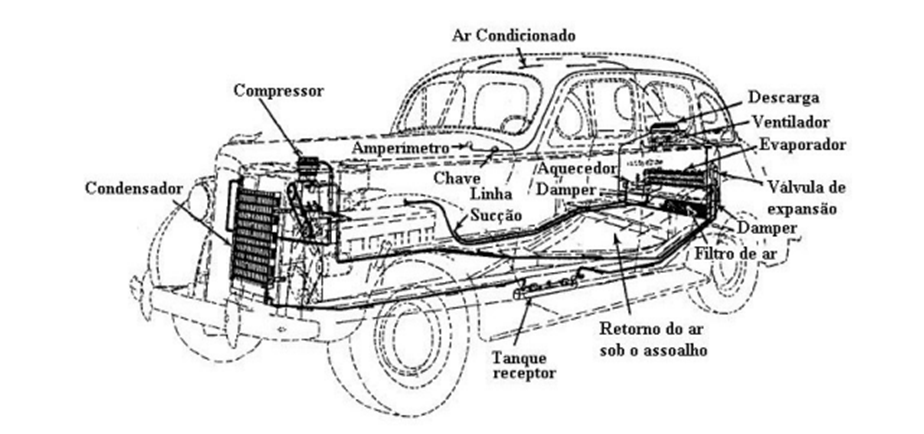
\includegraphics[width=15.65cm, height=7.35cm]{FigurasdoTexto/sistemaMAC.png}
    
     \vspace{5pt}  % Add space before source
    {\footnotesize Fonte: Bhatti adaptado por Santos (2005).}  % Source text in smaller font
    \label{fig:sistemaMAC}
\end{figure}

Atualmente, o Brasil está bem ranqueado na produção de veículos com sistema de condicionamento de ar nativo de fábrica, sendo o maior montador de veículos com ar condicionado da América do Sul e o 10º maior da América Latina com cerca de dois milhões de unidades de passeio \cite{dasilva2024}. Analisando o ano de novembro de 2024, a frota de veículos somente no Brasil era de 123,5 milhões, aproximadamente 63 milhões são automóveis, o que equivale a cerca de 51,2\%  \cite{ministerio2024}.

Esse sistema de condicionamento de ar automotivo consome uma parte significativa da potência do motor durante a operação do veículo, com sua eficiência de refrigeração diretamente relacionada à capacidade de carga térmica. Em média, o ar-condicionado é utilizado entre 43\% e 49\% do tempo total de uso do veículo \cite{farrington2000}.

O sistema por compressão mecânica de vapor utilizado em sistemas veiculares, segundo  \textcite{dasilva2016}, possui uma estrutura semelhante à dos sistemas de condicionamento de ar mecânico convencionais. Os principais componentes desses sistemas incluem trocadores de calor, um compressor e uma válvula ou dispositivo de expansão.

O princípio de funcionamento dos sistemas de condicionamento de ar e de refrigeração por compressão mecânica de vapor é compreendido pela operação dos quatro principais componentes: o compressor promove o escoamento do refrigerante ao longo do sistema, elevando a pressão e temperatura do fluido refrigerante, enquanto isso, o evaporador e condensador atuam como trocadores de calor, absorvendo e rejeitando o calor do ambiente a ser resfriado, e o dispositivo de expansão realiza a expansão isentrópica do fluido refrigerante, causando a redução da temperatura do mesmo \cite{junior2023}.

Em geral, as propriedades dos sistemas veiculares não permanecem constantes durante toda a operação de um veículo, sendo precedidas por um regime transitório em que as propriedades do sistema variam devido a fatores externos. Além disso, deve-se levar em conta o ciclo tradicional de controle da temperatura do veículo, no qual o sistema é acionado e desligado continuamente com o objetivo de atingir uma temperatura determinada \cite{juliani2017}.

Durante a operação nesse tipo de regime, os componentes podem apresentar não uniformidade das condições internas, a vazão mássica do refrigerante varia continuamente, resultando em mudanças na distribuição do refrigerante entre os componentes do sistema assim como a variação do superaquecimento e o ponto de operação do dispositivo de expansão, que se ajusta e regula continuamente para a operação \cite{rangel2007}. Devido a esse motivo, faz-se necessária a realização de mais estudos sobre o comportamento do sistema durante o regime transiente com o intuito de aumentar a eficiência do sistema de condicionamento de ar.

\subsection{OBJETIVOS}

\subsubsection{Objetivo Geral}

Análise experimental do comportamento transiente de um sistema de condicionamento de ar automotivo e de seu ciclo de histerese para avaliar o seu efeito sobre o coeficiente de performance (COP), considerando diferentes condições de operação.

\subsubsection{Objetivos Específicos}

Para alcançar o objetivo geral, os objetivos específicos propostos são:

\begin{enumerate}[label=\arabic*)]
    \item Revisão bibliográfica e obtenção de dados do sistema de referência;
    
    \item Identificar modos para controle da rotação do compressor;
    
    \item Adaptação do aparato experimental;
    
    \item Estimativa das incertezas experimentais;

    \item Elaboração do plano experimental;
    
    \item Realização dos experimentos e obtenção da base de dados experimental;
    
    \item Análise dos resultados.

\end{enumerate}
